\section{Performance}The HTCC is one of the major CLAS12 systems used in all experiments with electron beam and it provides a fast trigger signal. Therefore the efficiency of detecting scattered electrons is one of the critical parameters defining the quality of the data obtained in experiments. As shown in section VII the MC prediction has an efficiency of $\approx$100\% at a threshold of 3 phe. Fig.VIII-1 present the experimentally measured electron detection efficiency for elastically scattered electrons at 2 GeV. The corresponding applied thresholds were approximately 1-2 phe. Measurements were performed using a special procedure with a random trigger generated by a Faraday Cup (Charge-to-Frequency converted signal), which measured the charge accumulated during the experiment. As shown, the electron detection efficiency is $\eta$ = (99.6$\pm$0.3) \% which is in good agreements with the MC estimate.

\begin{figure*}
\begin{subfigure}[b]{0.49\textwidth}
    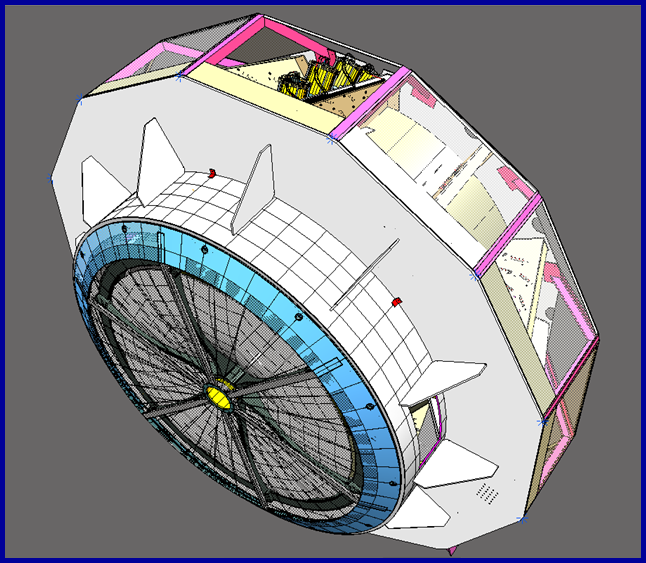
\includegraphics[width=0.9\textwidth]{Picture_3.png}
    \caption{First subfigure} \label{fig:subfig1_a}
\end{subfigure}
\hspace*{\fill} % separation between the subfigures
\begin{subfigure}[b]{0.49\textwidth}
    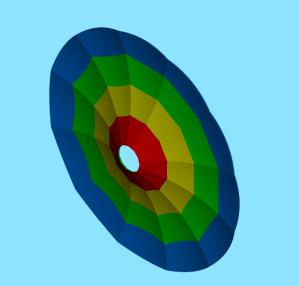
\includegraphics[width=0.9\linewidth]{ZERKALO.jpg}
    \caption{Second subfigure} \label{fig:subfig1_b}
\end{subfigure}
\caption{A figure that contains two subfigures} \label{fig:subfig1}
\end{figure*}

\begin{comment}
\begin{figure*}
    \centering
    \begin{minipage}[b]{0.49\textwidth}
        \centering
        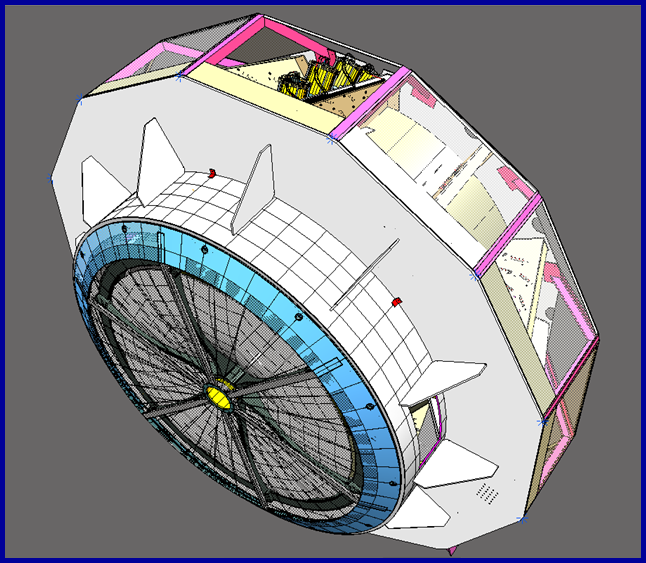
\includegraphics[width=0.9\textwidth]{Picture_3.png} % first figure itself
        \caption{first figure}
        \label{fig:my_label_A}
    \end{minipage}\hfill
    \begin{minipage}[b]{0.49\textwidth}
        \centering
        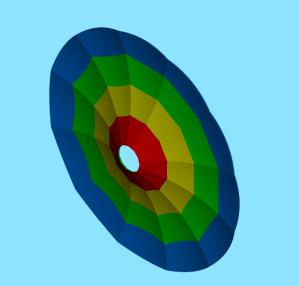
\includegraphics[width=0.9\textwidth]{ZERKALO.jpg} % second figure itself
        \caption{second figure}
        \label{fig:my_label_B}
    \end{minipage}
\end{figure*}
\end{comment}

\begin{comment}
\begin{figure}[h]
\centering
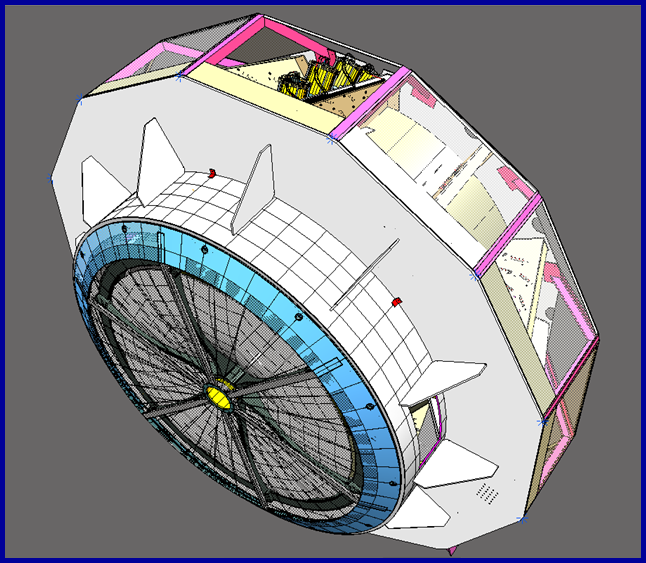
\includegraphics[width=0.75\linewidth]{Picture_3.png}
\caption{This is the first time using "Caption" option}
\label{fig:my_label}
\end{figure}
\end{comment}

\indent The signal strength in the HTCC, with the given design, depends on the actual properties of mirror facets, such as the final shape and reflectance, accuracy of the combined mirror assembly consisting of 60 mirror facets, accuracy of alignment (combined mirror, photomultiplier tubes), the composition of the radiator gas, and even on assembly technology (procedures). The ADC histograms of signal strength distribution obtained in all HTCC channels are shown in Fig.VIII-2. 

\begin{comment}
\begin{figure}[h]
\centering
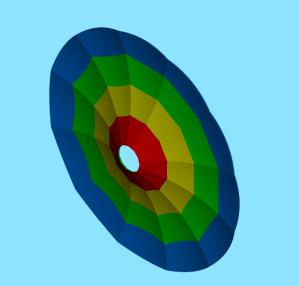
\includegraphics[width=0.75\linewidth]{ZERKALO.jpg}
\caption{Caption}
\label{fig:my_label}
\end{figure}
\end{comment}

Due to the different length of electron trajectories traveling in the working volume under different polar angles the statistics are lower for angles in range of 27.5$\degree$ to 35$\degree$. In particular we note that in cases when the electrons are crossing the mirror close to its edges (at approximately 5$\degree$ and 35$\degree$) one should expect unavoidable losses in the signal strength. As far as the “internal” borders between adjacent mirrors is concerned there are similar losses that of course take place and are finally compensated due to the complete azimuthal symmetry of the detector. As one can see there are differences between signal strengths in channels, which is to be expected. As mentioned above when discussing the assembly of the half-sector mirrors, the assembly and alignment of the combined mirror was done under tight control. This provided good results and final alignment of the PMT holding units, each which contain a photomultiplier tube, active and 3-layer passive magnetic shields, and a Winston Light Concentrator. The working gas composition was kept on the level of less than 100 ppm of water vapors by purging the volume at reasonable dry CO${_2}$ gas rates. The integrated signal strength is shown in Fig.VIII-3, and the average signal strength is about 16.5 phe.    

\indent Fig.VIII-4 present the results of the experimentally measured signal strength for all 60 mirror facets, which form a combined ellipsoidal mirror. One can see that there are areas along “internal” borders between adjacent mirror facets where signal strength is lower than average. This edge effect is unavoidable, i.e. is normal for the given design. We have discussed the possible changes in the shape of mirror facets due to shrinkage of the epoxy glue that was used in the combined mirror assembly. By applying the glue on the contact surfaces between facets in dots that do not touch each other we have prevented deformation in the direction along border between facets. But in the perpendicular direction, i.e. across thickness of the facets, there were only few glue dots and consequently the two outermost epoxy glue dots were not compensated for and their contribution to the deformation is significant since there are only 4-5 dots across the thickness. This effect can be visually observed by looking at the border between the two facets that are glued together. Even though the thickness of the glue joint is about 0.1 mm to 0.2 mm (the thickness of not reflecting area) and is insignificant when compared to the dimensions of the mirror facets, the deformed “wavy” edges of the facets glued together are estimated to be $\sim$5 mm. But since small deformations beyond the $\sim$5 mm band between mirrors do exist but are difficult to estimate their exact dimensions, then the final conservative conclusion of the influence of edge transverse deformation would be that the band’s width could be twice as wide. Apparently geometry of the mirror facets along those bands are different from designed. That difference in geometry directly leads to reduced light collection efficiency, i.e. to the reduction of signal strength.